% !TEX root = ../presentation.tex

\begin{frame}{Сравнение процессов обучения}
\begin{figure}
\centering
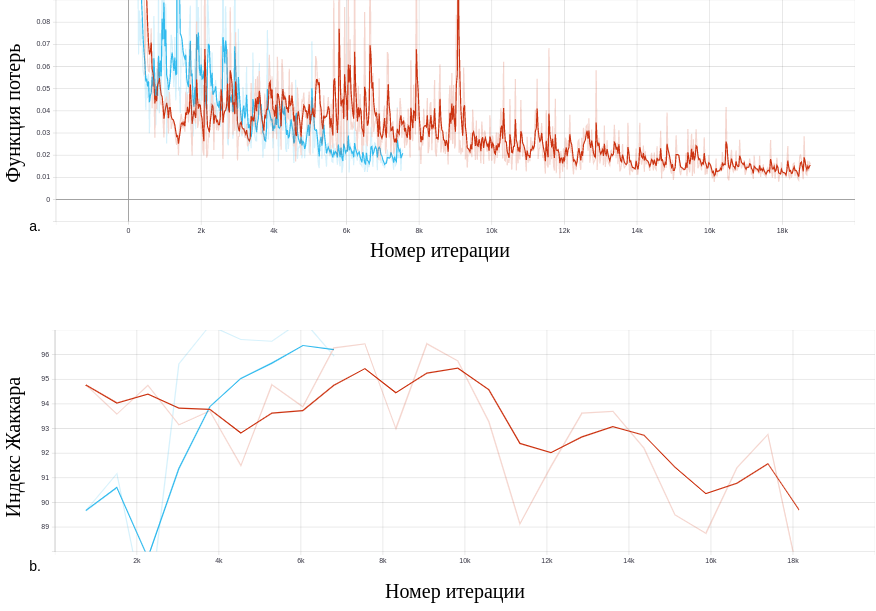
\includegraphics[width=8.76cm, height=6.11cm]{ocp_against_const.png}
\end{figure}
    Оранжевым отражен процесс обучения с постоянными значениями, голубым - с
    применением one cycle policy
%\textbf{$C$}-центр камеры (оптический центр); \textbf{$Cp$}-главная ось камеры
\end{frame}